\documentclass[twocolumn,a4paper]{article}

	% meta info goes here
	\author{
                F.M.S. Beekmans\\ ferdymoonsoobeekmans@gmail.com \\ 1327755
                A.J. Rouvoet\\ a.j.rouvoet@gmail.com \\ 4036964
                J. Bareman\\ jeroenbareman@gmail.com \\ 4035186}
	\title{Digital reconstruction of faded ink drawings}

	% package deps
	\usepackage{natbib}
	\usepackage{graphicx}

	% do not indent new paragraphs
	\setlength\parindent{0pt}

\begin{document}

	% use a one column layout
	% for the abstract, title and toc
	\twocolumn[
		\begin{@twocolumnfalse}
			\maketitle

			\begin{abstract}
				Here comes the abstract... with a test citation \cite{levin2004colorization}
			\end{abstract}

			\tableofcontents
		\end{@twocolumnfalse}
	]

	% include other sections of the paper here
	% introduction secion of the main paper
% it sets the context of our research and explains the goal of the paper
\section{Context}

	Many works of art deteriotate significantly over time.

	From an artistic point of view, it is of much interest to be able to view the drawings
	in the original coloring or, as one might say: in the way the artist intended the drawing.
	Paintings are often treated by curators to remove some of the pollution and regain
	the original properties.  Other works of art, of which the original is not recoverable by
	treating or cleaning the original piece (such as ink drawings), can be reproduced.
	Either on paper or digitally. \\

	Both of these recovery processes are time intensive and require a specialist's hand.
	And, when treating the original, it poses a risk of damaging the piece. \\

	We will specifically examine the recovery of the original coloring of ink drawings.
	Several types of detoriation occur with ink drawings:

	\begin{itemize}
		\item ink bleeding through from the backside of the drawing to the front
		\item ink color fading, due to light exposure
		\item paper decoloration, due to light exposure
	\end{itemize}

	The effects of above mentioned processes can be quite dramatic, as can be seen from
	figure \ref{montmajour}.

	\begin{figure}[h!]
		\label{montmajour}
		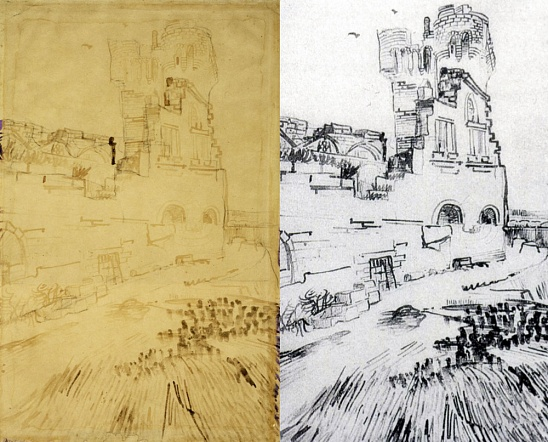
\includegraphics[width=\columnwidth]{graphics/montmajour}
		\caption{Reproduction of 'Montmajour' by Vincent van Gogh (1928) and a photographic reproduction}
	\end{figure}

	One might wonder how the original colors of a work can be determined.
	There are several sources that can tell us what the original colors where:

	\begin{itemize}
		\item margins of a drawing that were obscured from light by the frame
		\item (photographic) reproductions and/or facsimiles of the drawing
		\item similar drawings, of the same theme, same period or made with the same ink
	\end{itemize}

\section{Introduction}

	As mentioned before, the original can be reproduced digitally.
	A lot of time could potentially be safed if digital imaging techniques can be used to automate
	the recoloring of degraded work to the original colors.
	In the imaging field, a lot of techniques have been developed for retrieving information
	from images, recognizings patterns and color adjustments.
	Most of these techniques were not developed with art restauration as it's goal.
	Our research focusses on applying these existing methods to this specific problem. \\

	In this article we will examine a few of these techniques.
	We will discuss how these techniques can be applied to recover the original colors
	in faded ink drawings.
	Furthermore we will compare the techniques and based on that discussion formulate a possible
	method for digital reconstruction.

	% chapter about the `colorization using optimization` technique
\section{Colorization using optimization}
	
	Another technique for (re)coloring images is proposed by \citet{levin2004colorization}.
	They posed that any any pixel's color should not differ too much from the colors of it's 
	neighbours.
	That is: given any pixel, the difference between it's color and the weighted sum of it's
	neighbours colors should be minimal:

	\begin{equation}
		J(U) = \sum_r \left ( U(r) - \sum_{s \in N(r)} w_rs \cdot U(s) \right )^2
	\end{equation}

	Where $U(r)$ is the color of a pixel $r = (x,y)$ and $N(r)$ is the set of neighbours of $r$ 
	(any pixel in a given neighbourhood).
	The key in this equation is the weighting function $w_rs$.
	It determines how much the color of $r$ will be like the color of $s$.
	\citet{levin2004colorization} propose the use of two possible weighting functions,
	both relying on the luminance difference between $r$ and $s$.
	

        % comments and short explanation on the algorithm explained in "Fast
% Image and Video Colorization Using Chrominanche Blending"

\section{Fast Image and Video Colorization Using Chrominance
  Blending}

        In their paper \cite{yatziv2006fast} describe an algorithm to
        (re)colorize black and white images using scribbles thereon of color
        information\footnote{The supplied information is assumed to be correct
        however, this could also be an approximation of the correct color or
        location where this color should be.}. It is observed that in an
        original picture, the local difference in chrominance is roughly
        proportional to the local difference in luminance for each pixel.\\
        \\
        Based on this observation a simple algorithm is proposed. Every pixel
        that needs to be (re)colored will have the color of the weighed
        average of all the pixels in the scribble, where the weight is based
        on the geodesic distance to that pixel\footnote{Where each pixel is
        seen as a point $(x, y, Y)$ with $Y$ the luminance of the
        pixel.}.

        \subsection{applicability}
                This algorithm in it's current form seems too
                laborious to apply in the aforementioned context. It
                is likely that stricter assumptions can be made for
                monochramatic pictures, based on which this algorithm
                can be adapted for this problem. It is interesting to
                note that this is relatively insensitive to small
                errors introduced when manually placing the scribbles,
                this due to the use of geodesic distance as a weighing factor.
        
	% end of sections

	% use a one column layout
	% for the bibliography
	\twocolumn[
		\begin{@twocolumnfalse}
			\bibliographystyle{apalike}
			\bibliography{bibliography}
		\end{@twocolumnfalse}
	]

\end{document}
